\section{Rogue Class Weapons}

\subsubsection{The Kingslayers}

The Kingslayers are legend to be twin daggers that have been used in the assassination of multiple kings throughout ancient times.The blades are said to have been crafted by the legendary Hassassin (a rogue assassin trained from birth to be the perfect killing machine). The blades are believed to be infused with dark and poisonous magic that can corrupt anything they pierce. The blades are made from a rare metal that was mined from a meteorite. The blades are believed to have been traded down in generations within a small cult of specially trained Hassassins. The cult was focused on removing kings and nobles of high status if they did not fit their agendas. The blade is rumored to have vanished after the line of the Hassassins vanished during a world war when the planet divided its governments and broke into strife.

\begin{center}
	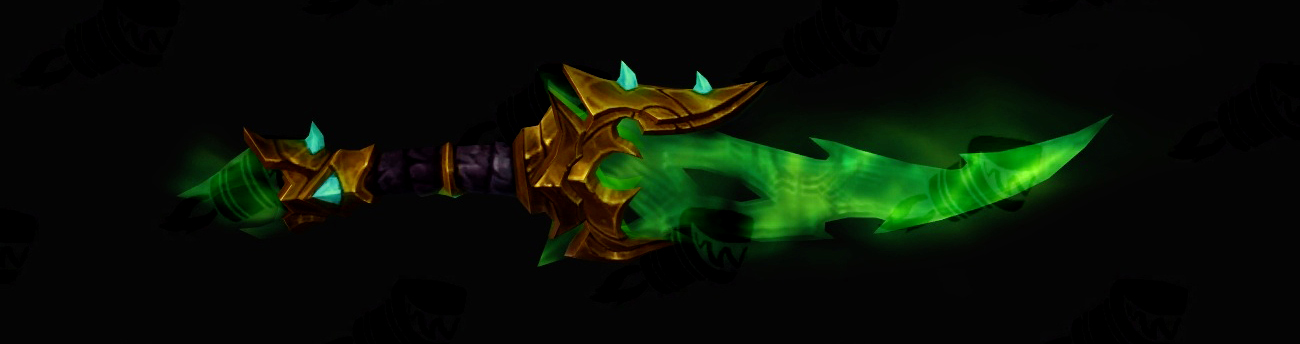
\includegraphics[width=\linewidth]{img/weapons/kingslayer-green.jpg}
	
	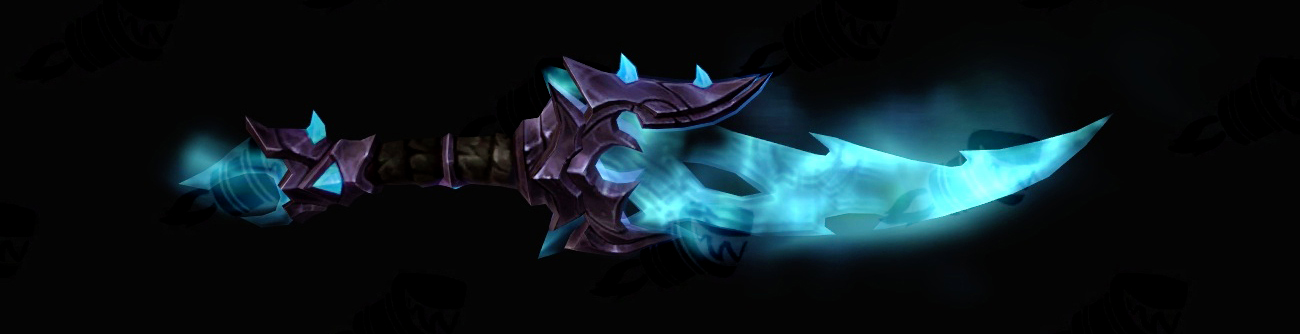
\includegraphics[width=\linewidth]{img/weapons/kingslayer-blue.jpg}
\end{center}

\subsubsection{Potential}

The Kingslayers want to remain hidden or be wielded by a member of the Hassassin bloodline. The Blades can sense the bloodline of their wielder and reject anyone not of the Hassassin descent. There are two blades and each have similar properties but different damage types.

\begin{commentbox}{Kingslayers\footnote{Weapon (daggers), artifact (requires attunement by a rogue)}}
	You gain a +3 bonus to attack and damage rolls made with this magic weapon. When you hit an enemy with the green blade you will deal 1d6 necrotic damage and 1d6 poison damage. When you hit an enemy with the blue blade you will deal 1d6 cold damage and 1d6 lightning damage. The damage will change to d10's if the target is not aware of the Rogues presence.
	
	The target of two successive attacks with both blades must make a constitution saving throw. On a fail, they take 5d6 poison damage. The DC for this save is the wielders level + their constitution.
	
	While a rogue wields The Kingslayers in combat it will look like the rogue has a shadowy presence. The wielder of the Kingslayers gains a +2 to stealth while wielding them.
	
	If a rogue of an non-Hassassin bloodline tries to attune to The Kingslayers they have to make a d20 roll. At a 18 or below The Kingslayers will reject you and deal 3d10 Poison damage and 2d10 Necrotic damage. At a 19 or 20 you over power the will of the weapon and make it yours.
	
	Proficiency with a daggers allows you to add your proficiency bonus to the attack roll for any attack you make with them.
	
	If the wielder of the Kingslayers dies, the Kingslayers will sink into the killer and attempt to kill it (unless it is within the Hassassin bloodline).
\end{commentbox}

\subsubsection{Finding The Kingslayers}

Within the Pluvian Realm, there exists an area referred to as crystal lake. This area is almost a perfect circle cut into the middle of the Pluvian wilderness. The region is a large flat lake that is iced over with multiple feet of thick ice. In the very center is a large fossilized pirate ship covered in ice. The wind is strong over this area and the air very cold. Surrounding the lake is forest. At the bottom of the ice in the depths of the river are solid crystals of various kinds. This gives the appearance of a shimmering surface when the sunlight is intense enough in this area.

The ship in the ice is frozen over with thick layers of ice. On the side of the ship is the name ``Charlotte'', which is the name of the ship. The ship and surrounding lake was frozen due to an Ice dragon that resides in a nearby cave. The ship contained the last Hassassin to wield the Kingslayers as well as the blades themselves. The Hassassin was not killed when the ship was frozen but rather preserved in the ice of the vessel. The Hassassin and the daggers are frozen within the hull of the ship alongside the Hassassin. If the vessel is thawed, it will come alive as will the frozen Hassassin. To obtain the Kingslayers one must kill the Hassassin.

\begin{center}	
	
\includegraphics[width=0.485\linewidth]{img/terrain/winter-frozen-lake-reflection-blue-ice-green-trees-wallpaper-quotes.jpg}
	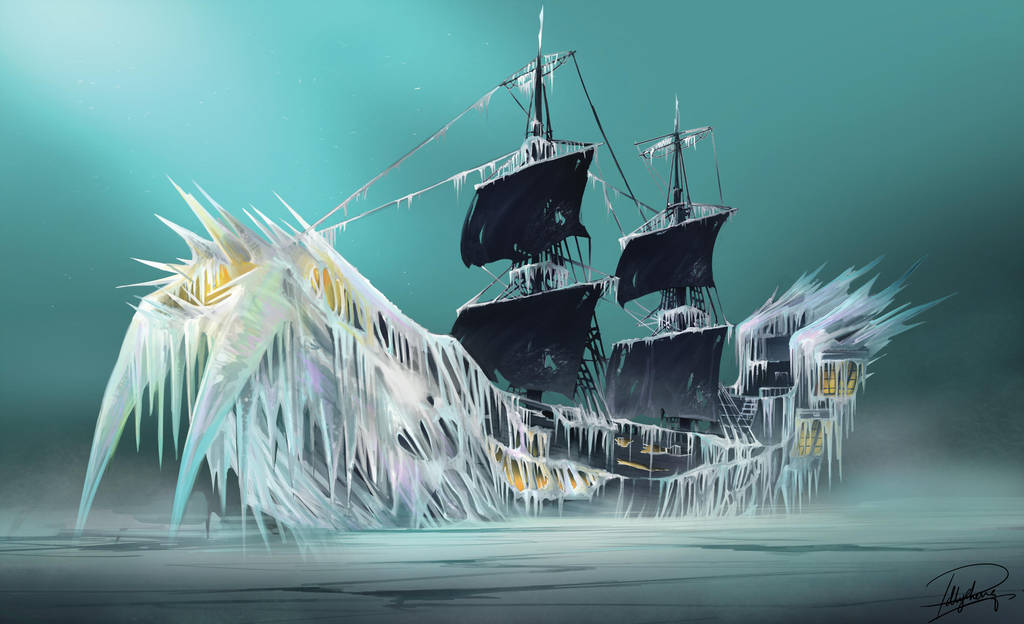
\includegraphics[width=0.50\linewidth]{img/ice_pirate_ship_by_pollychong_da47p92-fullview.jpg}
	
	\dndline
		
	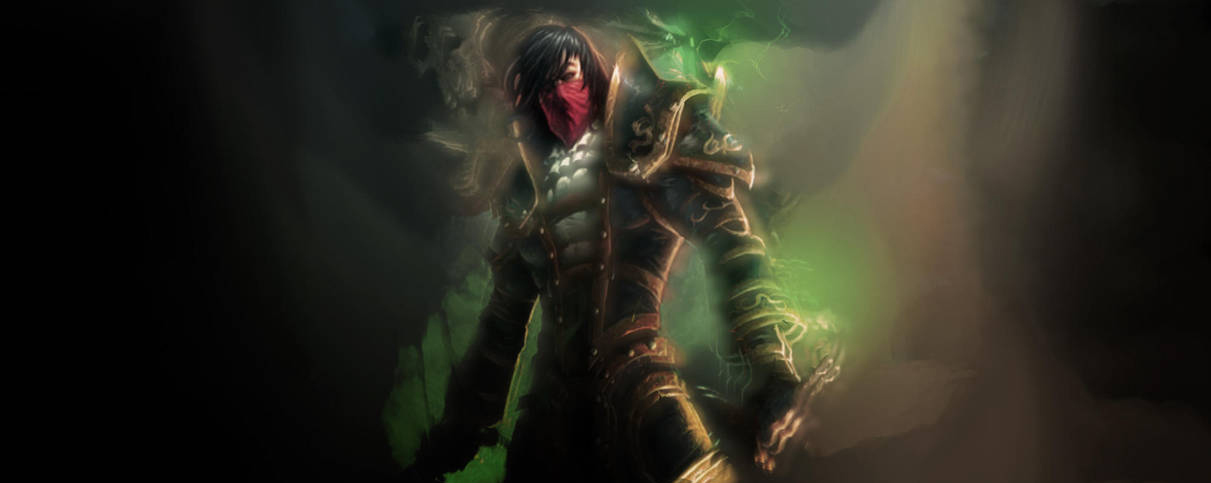
\includegraphics[width=\linewidth]{img/WoW/edwinvancleef.jpg}
\end{center}

\begin{monsterbox}{Weakened Hassassin}
	This character design is based on https://www.dndbeyond.com/monsters/assassin
	\begin{hangingpar}
		\textit{Medium humanoid, neutral evil}
	\end{hangingpar}
	\dndline%
	\basics[%
	armorclass = 16,
	hitpoints  = 98,
	speed      = 30 ft
	]
	\dndline%
	\stats[
	STR = \stat{11}, % This stat command will autocomplete the modifier for you
	DEX = \stat{18},
	CON = \stat{16},
	INT = \stat{13},
	WIS = \stat{11},
	CHA = \stat{10}
	]
	\dndline%
	\details[%
	% If you want to use commas in these sections, enclose the
	% description in braces.
	% I'm so sorry.
	languages = {Hassassin, Thieves' cant, Common},
	challenge = 10
	]
	\dndline%
	saving throws = DEX +7, INT +4
	
	skills = Acrobatics +6, Deception +3, Perception +3, Stealth +12
	
	damage resistance = Poison
	
	Senses = Passive Perception 13
	
	\dndline%
	\begin{monsteraction}[Assassinate]
		During its first turn or while vanished, the assassin has advantage on attack rolls against any creature that hasn't taken a turn. Any hit the assassin scores against a surprised creature is a critical hit.
	\end{monsteraction}	
	\begin{monsteraction}[Evasion]
		 If the assassin is subjected to an effect that allows it to make a Dexterity saving throw to take only half damage, the assassin instead takes no damage if it succeeds on the saving throw, and only half damage if it fails.		
	\end{monsteraction}	
	\begin{monsteraction}[Multiattack]
		The Hassassin makes two attacks.
	\end{monsteraction}
	\monstersection{Actions}
	\begin{monsteraction}[Kingslayer Attack]
		Melee Weapon Attack: +6 to hit, reach 5 ft., one target. Hit: See Kingslayer damage, replace the DC save effect with the following: the target must make a DC 15 Constitution saving throw, taking 24 (7d6) poison damage on a failed save, or half as much damage on a successful one.
	\end{monsteraction}
	\begin{monsteraction}[Light Crossbow]
		Ranged Weapon Attack: +6 to hit, range 80/320 ft., one target. Hit: 7 (1d8 + 3) piercing damage, and the target must make a DC 15 Constitution saving throw, taking 24 (7d6) poison damage on a failed save, or half as much damage on a successful one.
	\end{monsteraction}
	\monstersection{Legendary Actions}
	You can make 3 legendary actions per day. These are done after an action is done on any turn.
	\begin{monsteraction}[Vanish]
		You can magically wreath the area in smoke, vanishing from visibility. You remain concealed until performing an attack or successfully being perceived by another.
	\end{monsteraction}
\end{monsterbox}

